% TODO:
% - 

%%%%%%%%%%%%%%%%%%%%%%%%%%%%%%%%%%%%%%%%%%%%%%%%%%%%
% documentclss
\documentclass[]{beamer}
%\documentclass[handout]{beamer} %Drucker Version
%\documentclass[draft]{beamer}


%%%%%%%%%%%%%%%%%%%%%%%%%%%%%%%%%%%%%%%%%%%%%%%%%%%%
% packages

\usepackage[utf8]{inputenc}
\usepackage[ngerman]{babel}
\usepackage[T1]{fontenc}

\usepackage{setspace}
\usepackage{ellipsis}
\usepackage{microtype}
\usepackage{lmodern}

\usepackage{lscape}
\usepackage{booktabs}			% \toprule, \midrule und \bottomrule in Tabellen
\usepackage{multirow}
\usepackage{paralist}

%\usepackage{scrhack} 
\usepackage{listings}
\lstset{
    language=C,
    breaklines=true,
    breakatwhitespace=true
    basicstyle=\footnotesize,
    numbers=left,
    numberstyle=\footnotesize,
    stepnumber=1,
    numbersep=5pt,
    extendedchars=true,
    inputencoding=utf8,
    breakindent=30pt,
    escapeinside={\%(}{\%)},
    captionpos=b
}

%\usepackage[pdftex]{graphicx} % Bereits von Beamer geladen
\graphicspath{{../Master_Thesis/images/}}
\usepackage{tikz}
\usepackage{wrapfig}
\usepackage{caption}         
\usepackage{subcaption}      
\usepackage{pgfgantt}        
\usepackage{rotating} 		

\hypersetup{
    pdftex,
    bookmarks, bookmarksopen, bookmarksopenlevel=1, bookmarksnumbered=true,
    pdfpagemode={UseNone},
    pdfpagelayout={SinglePage},
    plainpages=false,
    pdfkeywords={AUTOSAR, Virtualisierung, ECU, Python, CAN},
    pdfsubject={Virtualisierung von AUTOSAR Softwarekomponenten für die Erprobung},
    pdftitle={Virtualisierung von AUTOSAR Softwarekomponenten für die Erprobung},
    pdfauthor={Martin Wichmann},
}



\newcommand{\inputImage}[1]{\input{../Master_Thesis/images/#1}}
% Bild einfügen:
%\centering
%\resizebox{0.3\linewidth}{!}{\inputImage{autosar_overview.dia}}

\newtranslation[to=ngerman]{Example}{Beispiel}

\usetheme{Warsaw}

\AtBeginSection[]
{
   \begin{frame}
        \frametitle{Inhaltsübersicht}
        \tableofcontents[currentsection,hideallsubsections]
   \end{frame}
}



%%%%%%%%%%%%%%%%%%%%%%%%%%%%%%%%%%%%%%%%%%%%%%%%%%%%
% Title
\author{Martin Wichmann}
\title[Virtualisierung von AUTOSAR Softwarekomponenten]{Virtualisierung von AUTOSAR Softwarekomponenten für die Erprobung}
\subtitle{Kolloquium zur Masterarbeit}
\date{\today}
\institute{Ostfalia Hochschule für angewandte Wissenschaften}




%%%%%%%%%%%%%%%%%%%%%%%%%%%%%%%%%%%%%%%%%%%%%%%%%%%%
% begin document
\begin{document}

\begin{frame}
\maketitle
\end{frame}


\begin{frame}
\frametitle{Inhaltsübersicht}
\tableofcontents[hideallsubsections] % Einstellungen siehe Beamer User Guide Seite 99
\end{frame}





%%%%%%%%%%%%%%%%%%%%%%%%%%%%%%%%%%%%%%%%%%%%%%%%%%%%%%%%%%%%%%%%%%%5
% Einleitung
\section{Einleitung}
\label{sec:einleitung}

%%%%%
\begin{frame}
\frametitle{Einleitung}
    \begin{itemize}
        \item AUTOSAR mittlerweile etabliert
        \item Virtualisierung im Server-Bereich üblich
        \item In dieser Arbeit:
        \begin{itemize}
            \item Evaluation von Virtualisierung im Embedded-Bereich
            \item Evaluation von AUTOSAR
        \end{itemize}
        \item Einsatzbereiche
        \begin{itemize}
            \item Lehre und Evaluation
            \item Reale Projekte
        \end{itemize}
        \item Schwerpunkt: Kommunikation und Virtualisierung
    \end{itemize}
\end{frame}


%%%%%%%%%%
%\subsection{Zielsystem}

%%%%%
\begin{frame}
\frametitle{Motivation}
    \begin{figure}[ht]
        \centering
        \resizebox{0.9\linewidth}{!}{\inputImage{arch_begin.dia}}
        \caption{Fallbeispiel}
        \label{fig:fallbeispiel}
    \end{figure}
\end{frame}



%%%%%%%%%%%%%%%%%%%%%%%%%%%%%%%%%%%%%%%%%%%%%%%%%%%%%%%%%%%%%%%%%%%5
% Grundlagen
\section{Grundlagen}
\label{sec:grundlagen}

%%%%%%%%%%
\subsection{Virtualisierung}
%%%%%
\begin{frame}
\frametitle{Überblick}
    \begin{itemize}
        \item Beschreibt eine Reihe von Techniken
        \item Ein reales System --> mehrere virtuelle Systeme
        \item Zentrales Element: Hypervisor
        \item Verschiedene Ziele:
        \begin{itemize}
            \item Zugriff auf verschiedene Betriebssysteme
            \item Wartbarkeit
            \item Skalierbarkeit
            \item Ausfallsicherheit
        \end{itemize}
    \end{itemize}
\end{frame}

%%%%%
\begin{frame}
\frametitle{Hypervisor Kategorien}
    \begin{figure}
        \centering
        \begin{subfigure}[b]{0.49\textwidth}
            \centering
            \resizebox{0.9\linewidth}{!}{\inputImage{virt_type1.dia}}
            \caption{Type 1-Hypervisor}
            \label{fig:hypervisor_type1}
        \end{subfigure}
        \begin{subfigure}[b]{0.49\textwidth}
            \centering
            \resizebox{0.9\linewidth}{!}{\inputImage{virt_type2.dia}}
            \caption{Type 2-Hypervisor}
            \label{fig:hypervisor_type2}
        \end{subfigure}
        \caption{Hypervisor Kategorien}
        \label{fig:hypervisor}
    \end{figure}
\end{frame}

%%%%%
\begin{frame}
\frametitle{Virtualisierung in eingebetteten Systemen}
    \begin{itemize}
        \item Auch bekannt als: \emph{Time and Space Partitioning}
        \item SOCs immer leistungsfähiger
        \item Automobil: Bis zu 50 Steuergeräte
        \item Spezielle Anforderungen
        \begin{itemize}
            \item Energieverbrauch
            \item Speichernutzung
            \item Sicherheit
            \item Determinismus und Echtzeitfähigkeit
        \end{itemize}
        \item Bereits im Einsatz: ARINC 653
    \end{itemize}
\end{frame}


%%%%%
\begin{frame}
\frametitle{ARINC 653 Übersicht}
    \begin{figure}[ht]
        \centering
        \resizebox{0.65\linewidth}{!}{\inputImage{arinc653.dia}}
        \caption{ARINC 653 Architektur Übersicht}
        \label{fig:arinc_653}
    \end{figure}
\end{frame}

%%%%%
\begin{frame}
\frametitle{Marktübersicht}
    \begin{itemize}
        \item PikeOS
        \item OKL4 Microvisor
        \item INTEGRITY Multivisor
        \item COQOS
        \item XtratuM
    \end{itemize}
\end{frame}

%%%%%
\begin{frame}
\frametitle{Vorteile und Nachteile}
    \begin{itemize}
        \item[$ + $] Unabhängigkeit vom Betriebssystem
        \item[$ + $] Sicherheit
        \item[$ + $] Wiederverwenden von altem Code
        \item[$ + $] IP-Schutz und Trennung von Software-Lizenzen
        \item[$ + $] Hypervisor klein und robust

        \item[$ - $] Single Point of Failure
        \item[$ - $] Leistungseinbußen
        \item[$ - $] Größere Folgen eines Ausfalls
    \end{itemize}
\end{frame}


%%%%%%%%%%
\subsection{AUTOSAR}

%%%%%
\begin{frame}
\frametitle{AUTOSAR Einleitung}
    \begin{itemize}
        \item AUTomotive Open System ARchitecture
        \item Systemarchitektur
        \item Entwicklungsmodell
        \item Entwickelt von und für die Automobilindustrie
        \item "`Erbe"' von OSEK/VDX
        \item AUTOSAR ist nur Standard und beschreibt Schnittstellen
    \end{itemize}
\end{frame}

%%%%%
\begin{frame}[plain]
\frametitle{AUTOSAR Überblick}
    \begin{figure}[p]
        \centering
        \resizebox{0.6\linewidth}{!}{\inputImage{autosar_overview.dia}}
        \caption{Autosar Überblick}
        \label{fig:autosar_overview}
    \end{figure}
\end{frame}

%%%%%
\begin{frame}
\frametitle{Grundkonzepte}
    \begin{itemize}
        \item Systembeschreibung (System Description)
        \item Kommunikationsinformationen
        \item Quellcode und Objektdateien
        \item AUTOSAR Entwicklungswerkzeug
        \begin{itemize}
            \item Basis-Software-Implementation
            \item Basis-Software-Konfigurator
            \item Runtime-Enviroment-Generator
        \end{itemize}
    \end{itemize}
\end{frame}

%%%%%
\begin{frame}
\frametitle{Entwicklungsprozess}
    \begin{figure}[ht]
        \centering
        \resizebox{0.98\linewidth}{!}{\inputImage{Autosar_Prozess.dia}}
        \caption{AUTOSAR-Entwicklungsprozess}
        \label{fig:autosar_prozess}
    \end{figure}
\end{frame}

%%%%%
\begin{frame}
\frametitle{AUTOSAR-Schichtenmodell}
    \begin{figure}[ht]
        \centering
        \resizebox{0.98\linewidth}{!}{\inputImage{autosar_layer.dia}}
        \caption{AUTOSAR-Schichtenmodell}
        \label{fig:autosar_layer}
    \end{figure}
\end{frame}

%%%%%
\begin{frame}[fragile]
\frametitle{VFB und RTE}
    \begin{itemize}
        \item Virtual Functional Bus --> Designphase
        \item Runtime-Enviroment --> Compilephase
        \item 1 VFB pro System --> 1 RTE pro ECU
        \item Trennung zwischen Applikation und Basissoftware
        \item Schnittstellen/Interfaces werden in VFB definiert
    \end{itemize}
    \begin{exampleblock}{Beispiel Sender/Receiver-Interface}
        \begin{verbatim}
Rte_Write_<p>_<d>(self, data)
Rte_Read_<p>_<d>(self, data)
        \end{verbatim}
    \end{exampleblock}
\end{frame}


%%%%%
\begin{frame}
\frametitle{Basissoftware}
    \begin{itemize}
        \item "`Betriebssystem"'
        \item Modular
        \item Statisches System
        \item Schnittstellen sowie Umfang der Module festgelegt
        \item Granularität: Implementation Conformance Classes
        \item Wichtige Module: Os, SchM, Com, PduR
    \end{itemize}
\end{frame}


%%%%%
\begin{frame}
\frametitle{AUTOSAR-Schichtenmodell mit Modulen}
    \begin{figure}[ht]
        \centering
        \resizebox{0.98\linewidth}{!}{\inputImage{autosar_refined_layer.dia}}
        \caption{AUTOSAR-Schichtenmodell mit genauerer Aufteilung}
        \label{fig:autosar_refined_layer}
    \end{figure}
\end{frame}

%%%%%
\begin{frame}
\frametitle{Kritik an AUTOSAR}
    \begin{itemize}
        \item Effizienz
        \item Umfang des Standards
        \item Schnelle Entwicklung von AUTOSAR
        \item Bindung an Hersteller
        \item Starke Relevanz der Designphase
        \item Dokumentation der Konfiguration
        \item Portabilität von Softwarekomponenten
    \end{itemize}
\end{frame}




%%%%%%%%%%
\subsection{Netzwerkmanagment}
%%%%%
\begin{frame}
\frametitle{Netzwerkmanagement}
    \begin{itemize}
        \item Synchroner Wechsel des Buszustands
        \item Ziele: Energie sparen, Fehler vermeiden
        \item Implementation nicht allgemein spezifiziert
        \item Allgemein: Braodcastbotschaften geben Zustand einer ECU bekannt
        \item Mögliche Konzepte:
        \begin{itemize}
            \item Direktes Monitoring
            \item Indirektes Monitoring
            \item Master/Slave
            \item Peer-to-Peer
        \end{itemize}
    \end{itemize}
\end{frame}



% TODO: soll das rein?! Wenn ja in welchem Umfang?!
%%%%%%%%%%
%\subsection{Funktionale Sicherheit}
%%%%%
%\begin{frame}
%\frametitle{TODO}
%    \begin{itemize}
%        \item Allgemeiner, methodischer Ansatz zu Absicherung
%        \item DIN/IEC 61508
%        \item ISO 26262
%        \begin{block}{TODO}
%Die Ersatzpflicht des Herstellers ist ausgeschlossen, wenn [\dots] der Fehler nach dem Stand der Wissenschaft und Technik in dem Zeitpunkt, in dem der Hersteller das Produkt in den Verkehr brachte, nicht erkannt werden konnte.
%        \end{block}
%    \end{itemize}
%\end{frame}







%%%%%%%%%%%%%%%%%%%%%%%%%%%%%%%%%%%%%%%%%%%%%%%%%%%%%%%%%%%%%%%%%%%5
% Umsetzung
\section{Umsetzung}
\label{sec:umsetzung}

% TODO: Anforderungen an Fallbeispiel
%%%%%
\begin{frame}
\frametitle{Überblick}
    \begin{figure}[ht]
        \centering
        \resizebox{0.8\linewidth}{!}{\inputImage{arch_finished.dia}}
        \caption{Vollständige Architektur}
        \label{fig:arch_finished}
    \end{figure}
\end{frame}




%%%%%%%%%%
\subsection{Virtualisierung}
%%%%%
\begin{frame}
\frametitle{Virtualisierung}
    \begin{itemize}
        \item 2 VMs
        \begin{itemize}
            \item AUTOSAR-Komponente
            \item VCAN-Applikation
        \end{itemize}
        \item Hypervisor
        \begin{itemize}
            \item Fallbeispiel: Type 2 --> VirtualBox
            \item Evaluation: Type 1 --> XtratuM
        \end{itemize}
    \end{itemize}
\end{frame}

%%%%%
\begin{frame}
\frametitle{XtratuM}
    \begin{itemize}
        \item Open-Source Type 1-Hypervisor
        \item Universitat Politècnica de València (Spanien)
        \item Angelehnt an ARINC-653
        \item Arbeitsfluss:
        \begin{itemize}
            \item XML-Konfiguration
            \item C-Code
            \item Kompilieren
        \end{itemize}
    \end{itemize}
\end{frame}


%%%%%%%%%%
\subsection{Kommunikation Linux und AUTOSAR}
%%%%%
\begin{frame}
\frametitle{Kommunikationstechniken}

    \begin{itemize}
        \pause
        \item Interprozesskommunikation
        \begin{itemize}
            \item[$ + $] Geringer Overhead
            \item[$ - $] Nicht in AUTOSAR vorgesehen
        \end{itemize}
        \pause
        \item CAN
        \begin{itemize}
            \item[$ + $] Standard im Embedded-Bereich
            \item[$ - $] Hardware für jedes System nötig
        \end{itemize}
        \pause
        \item Ethernet
        \begin{itemize}
            \item[$ + $] Standard in allgemeiner Übertragungstechnik
            \item[$ - $] Erst ab AUTOSAR 4.0 unterstützt
        \end{itemize}
        \pause
        \item VCAN
        \begin{itemize}
            \item[$ + $] Baut auf Ethernet auf
            \item[$ - $] Auf EB tresos beschränkt
        \end{itemize}
    \end{itemize}

\end{frame}

%%%%%
\begin{frame}
\frametitle{VCAN}
    \begin{itemize}
        \item Ethernet TCP-Verbindung
        \item Format
        \begin{itemize}
            \item System
            \item Kanal
            \item CAN-Botschaft --> ID, DLC, Daten
        \end{itemize}        
        \item Gateway nötig
        \item VCAN-API
        \begin{itemize}
            \item In Python realisiert
            \item Gateway-API
            \item Client-API
            \item Erweiterbar --> Zugriffskontrolle
        \end{itemize}
    \end{itemize}
\end{frame}




%%%%%%%%%%
\subsection{Kommunikation AUTOSAR und Scheinwerfer-ECU}
%%%%%
\begin{frame}
\frametitle{Steuergerät}
    \begin{itemize}
        \item Bisheriges Steuergerät
        \begin{itemize}
            \item Low-Speed-CAN
            \item Altes Netzwerkmanagement --> Von EB tresos nicht untersützt
        \end{itemize}
        \item Aktuelles Steuergerät
        \begin{itemize}
            \item EB tresos Netzwerkmanagement unterstützt
            \item Funktionalität teilweise durch CRC geschützt
            \item CRC-Werte durch Restbussimulation ermittelt
        \end{itemize}
    \end{itemize}
\end{frame}


%%%%%
\begin{frame}
\frametitle{AUTOSAR Netzwerkmanagment}
    \begin{exampleblock}{NM-Botschaften}
        \begin{table}
        \centering
            \begin{tabular}[h]{l l l}
                Node & ID & Botschaft\\
                \toprule
                SMLS        & 0x1B00000C & 0C:00:04:00:00:00:00:00\\
                BCM         & 0x1B00000E & 0E:00:04:01:11:00:0C:00\\
                ---         & 0x1B000010 & 10:00:04:00:00:00:00:00\\
                ---         & 0x1B000014 & 14:00:04:00:00:00:00:00\\
            \end{tabular}
        \label{tab:jitter_statistik}
        \end{table}
    \end{exampleblock}
    \begin{itemize}
        \item Byte 1: Source Node Identifier
        \item Byte 2: Control Bit Vector
        \item Rest: Nutzdaten --> VW-eigenes Protokoll
    \end{itemize}
\end{frame}




%%%%%%%%%%
\subsection{Entwicklung AUTOSAR-Komponente}
%%%%%
\begin{frame}
\frametitle{Systemmodell AUTOSAR-Komponente}
    \begin{figure}[ht]
        \centering
        \resizebox{\linewidth}{!}{\inputImage{SMLS_Modell.dia}}
        \caption{Entwickeltes Komponenten Modell}
        \label{fig:smls_modell}
    \end{figure}
\end{frame}




%%%%%%%%%%
\subsection{Entwicklung steuernde Komponente}
%%%%%
\begin{frame}
\frametitle{Steuernde Komponente}
    \begin{itemize}
        \item Basiert auf VCAN-API
        \item Zugriff auf Signale
        \item Übersichtliche Darstellung des Zustands
    \end{itemize}
\end{frame}

%%%%%
\begin{frame}
\frametitle{Demonstration}

\end{frame}





%%%%%%%%%%%%%%%%%%%%%%%%%%%%%%%%%%%%%%%%%%%%%%%%%%%%%%%%%%%%%%%%%%%5
% Fazit
\section{Analyse und Fazit}
\label{sec:analyse_fazit}

%%%%%%%%%%
\subsection{Analyse}
%%%%%
\begin{frame}
\frametitle{Relevanz für reale Projekte}
    \begin{itemize}
        \item Infotainment und Fahrerassistenzsysteme
        \item Anbindung an Internet oder Car2X
        \item Virtualisierung wird bereits in Avionik und Mobilfunkbranche eingesetzt
        \item Funktionale Sicherheit beschränkt auf VMs
        \item Produktivcode als Restbussimulation
        \item VCAN bietet einfachen Zugriff
    \end{itemize}
\end{frame}

%%%%%
\begin{frame}
\frametitle{Benchark und Echtzeitfähigkeit}
    \begin{figure}
        \centering
        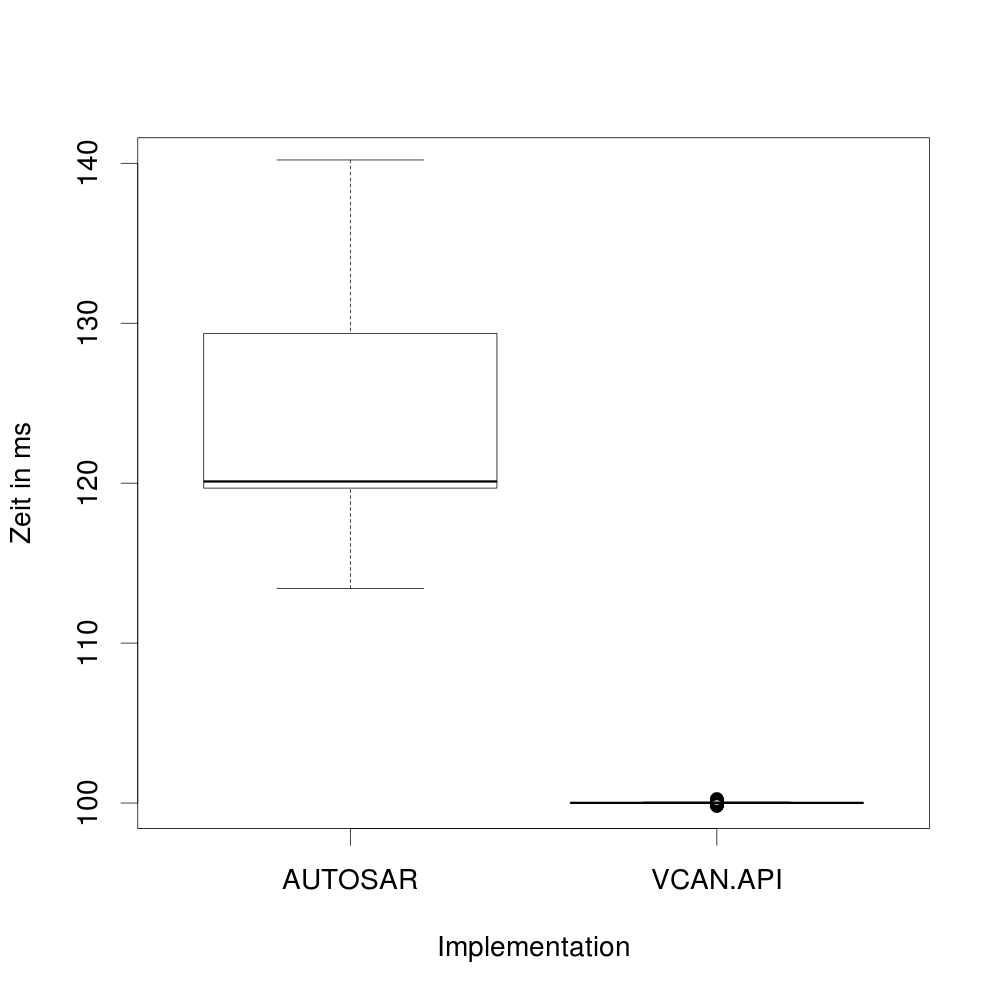
\includegraphics[width=0.5\textwidth]{boxplot}
        \caption[Zeitanalyse des VCAN als Boxplots]{Zeitanalyse des VCAN als Boxplots}
        \label{fig:timinganalyse}
    \end{figure}
\end{frame}

%%%%%
\begin{frame}
\frametitle{Sicherheitsbetrachtung der Virtualisierung}
    \begin{itemize}
        \item Angriffssicherheit
        \begin{itemize}
            \item Gleiche Probleme klassischen Systemen
            \item Angriffsweg Internet
        \end{itemize}
        \pause
        \item Betriebssicherheit
        \begin{itemize}
            \item Verteiltes System --> Vereinigtes System
            \item Weniger Hardware Redundanz
        \end{itemize}
        \pause
        \item Absicherung der Kommunikation
        \begin{itemize}
            \item Integrität und Authentizität durch signieren und verschlüsseln
            \item AUTOSAR 4.0 bietet \emph{Crypto Service}
            \item Dedizierte VM kann Service anbieten (SSL, RSA, MD5\dots)
        \end{itemize}
    \end{itemize}
\end{frame}


%%%%%%%%%%
\subsection{Fazit und Ausblick}
%%%%%
\begin{frame}
\frametitle{Fazit}
    \begin{itemize}
        \item Virtualisierung ist ausgereiftes Konzept
        \begin{itemize}
            \item Erhöhte Komplexität
            \item Verbesserte Abstraktion
            \item Type 1-Hypervisor für Vorteile notwendig
        \end{itemize}
        \item WinCore und VCAN
        \begin{itemize}
            \item Guter Einstieg
            \item Instabilität kritisch
        \end{itemize}
        \item AUTOSAR
        \begin{itemize}
            \item Notwendiger Schritt
            \item Zu komplex?
        \end{itemize}
        % TODO: ISO 26262 notwendig
    \end{itemize}
\end{frame}


%%%%%
\begin{frame}
\frametitle{Ausblick}
    \begin{itemize}
        \item XtratuM in der Lehre
        \item VCAN
        \begin{itemize}
            \item VCAN-API erweiterbar
            \item DBC, ARXML Unterstützung
            \item Restbussimulation
            \item \dots
        \end{itemize}
    \end{itemize}
\end{frame}










%%%%%%%%%%%%%%%%%%%%%%%%%%%%%%%%%%%%%%%%%%%%%%%%%%%%%%%%%%%%%%%%%%%5
% Literaturangaben
\appendix
\section*{Literatur}
\label{sec:Literatur}

\begin{frame}


\begin{thebibliography}{10}

\bibitem[1]{1} \textsc{Olaf Kindel, Mario Driedrich}: {\em Softwareentwicklung mit AUTOSAR: Grundlagen, Engineering, Management in der Praxis.} dpunkt.verlag, 2009.

\bibitem[2]{2} \textsc{Peter Löw, Roland Pabst, Erwin Petry}: {\em Funktionale Sicherheit in der Praxis.} dpunkt.verlag, 2010.

\bibitem[3]{3} \textsc{AUTOSAR}: {\em Technical Overview.} Online unter: \url{http://autosar.org/download/R3.1/AUTOSAR_TechnicalOverview.pdf}

\bibitem[4]{4} \textsc{AUTOSAR}: {\em Layered Software Architecture.} Online unter: \url{http://autosar.org/download/R3.1/AUTOSAR_LayeredSoftwareArchitecture.pdf}

\end{thebibliography}


\end{frame}

\end{document}

